\section{Neural Networks and Deep Learning}

%%%%%%%%%%%%%%%%%%%%%%%%%%%
%%%%%%%%%%%%%%%%%%%%%%%%%%%
%%%%%%%%%%%%%%%%%%%%%%%%%%%
%%%%%%%%%%%%%%%%%%%%%%%%%%%
%%%%%%%%%%%%%%%%%%%%%%%%%%%
\subsection{Introduction}

A neural network is a ML model inspired by the network of biological neurons in our brains.

NNs are versatile, powerful, and scalable.
Consequently, they frequently outperform other ML techniques on very large and complex problems.
NNs are at the very core of Deep Learning.

\textbf{Threshold Logic Units (TLUs)} are the building block of neural networks (i.e. the neurons):
\begin{itemize}
\vspace{-4.0mm}

\item
First, they perform a weighted sum of the inputs, $z = \sum w_i x_i$

\item
\vspace{-2.0mm}
Then they apply an \textit{activation function} to that sum, $h_{\boldsymbol{w}}(\boldsymbol{x}) = \phi(z)$, and output the result.\newline
\begin{figure}[ht]
\centering
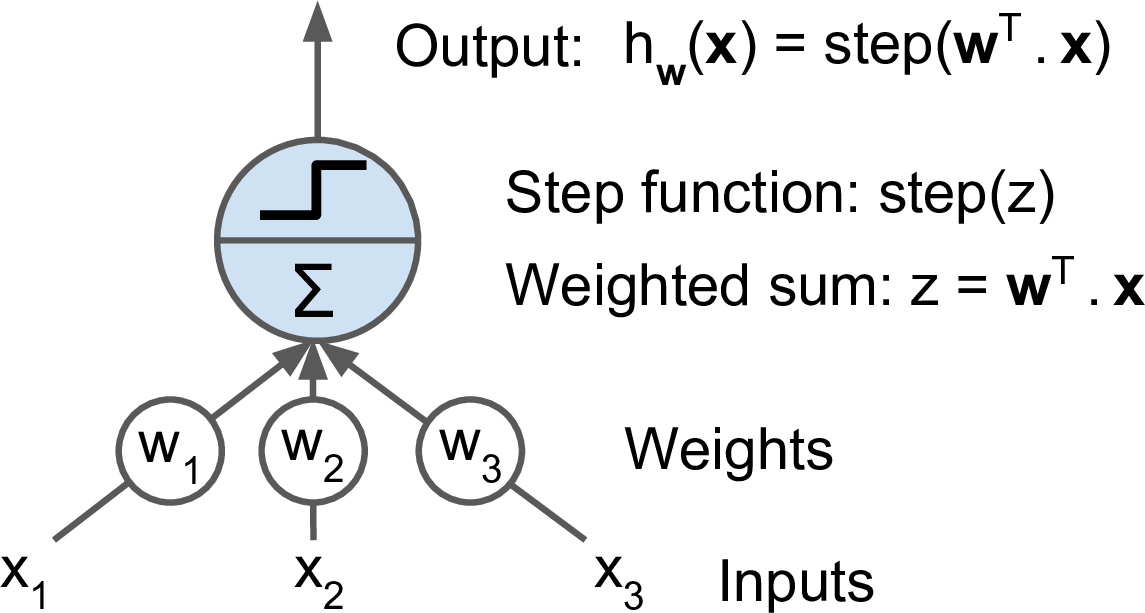
\includegraphics[width=0.50\textwidth]{./images/TLU.png}
\end{figure}

\item
\vspace{-2.0mm}
Traditionally, the activation function was a heavyside step function.
However, in order to perform Gradient Descent on a NN,
a differentiable function was needed instead.\newline
- The default has become the Rectified Linear Unit functoin: ReLU(z) = max(0,z)\newline
- The logistic function and hyperbolic tangent function are also popular choices.
\end{itemize}
\vspace{-2.0mm}


\textbf{Multilayer Perceptrons (MLPs)} are composed of multiple TLUs as depicted in the diagram.\newline
\textit{The bias neurons are shown, but usually they are implicit.}
\begin{figure}[ht]
\centering
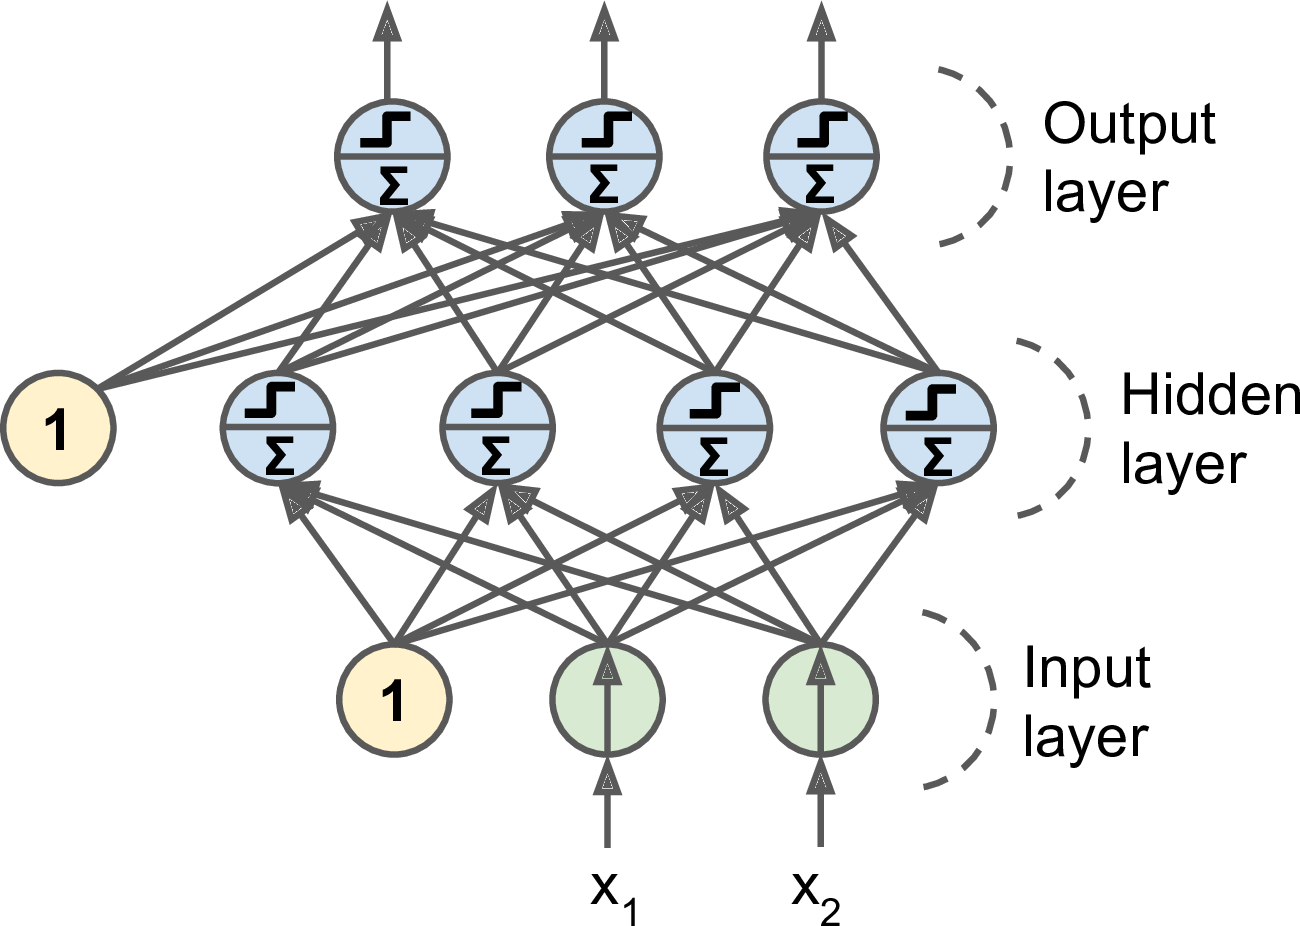
\includegraphics[width=0.50\textwidth]{./images/MLP.png}
\end{figure}

\vspace{-6.0mm}
\begin{itemize}
\item
When there's a deep stack of hidden layers, it is called a \textit{deep neural network (DNN)}.
\item
\vspace{-2.0mm}
Layers close to the input layer are called the \textit{lower layers}\newline
Layers close to the output layer are called the \textit{upper layers}.
\item
\vspace{-2.0mm}
When all the neurons in a layer are connected to every neuron in the previous layer,\newline
the layer is called a \textit{fully connected layer} or a \textit{dense layer}.
\item
\vspace{-2.0mm}
The signal flows only in one direction $=$ \textit{feedforward neural network (FNN)}.
\item
\vspace{-2.0mm}
Without the activation functions, all you would get is a linear model!
\end{itemize}

\newpage
\textbf{Training NNs: Backpropagation}.\newline
In just two passes through the network (one forward, one backward)
the backpropagation algorithm is able to compute the gradient of the network's error
with regard to every single model parameter (i.e. the connection weights),
allowing Gradient Descent to be used to train the NN.

\vspace{-5.0mm}
\begin{itemize}
\item
It handles one mini-batch at a time. The bigger the batch size, the more memory required.

\item
\vspace{-2.0mm}
\textit{The forward pass}.
Each mini-batch is passed through the network.
The output of every neuron is computed and preserved (for every instance in the mini-batch).

\item
\vspace{-2.0mm}
The network's output error is measured.

\item
\vspace{-2.0mm}
\textit{The reverse pass}.
The error gradient across all the connection weights is measured
by propagating the error gradient backward through the network.

\item
\vspace{-2.0mm}
an \textbf{iteration} = one forward-backward pass using one mini-batch.\newline
an \textbf{epoch} = one forward-backward pass of \textit{all} the training set examples.\newline
If you have 2000 training examples, and your batch size is 500\newline
$\rightarrow$ then it will take 4 iterations to complete 1 epoch.

\item
\vspace{-2.0mm}
It is important to randomly initialize all the hidden layer's connection weights.\newline
This breaks the symmetry and allows backpropagation to train a diverse team of neurons.

\end{itemize}

\textbf{Regression MLPs: Summary}

\begin{tabular}{ |l|l| } 
\hline
Hyperparameter & Typical value \\ 
\hline
Number of input neurons & One per input feature \\ 
Number of hidden layers & Depends on the problem, but typically 1 to 5\\ 
Number of neurons per hidden layer & Depends on the problem, but typically 10 to 100\\ 
Hidden layer activation function & ReLU or SELU\\
Number of output neurons & 1 per prediction dimension\\
Output activation function & In general None (can output any range of values)\\
 & ReLU/softplus (for a positive output contraint)\\
 & Logistic/tanh (for a bounded output contraint)\\
Loss function & Typically MSE (mean squared error)\\
 & Maybe MAE (mean absolute error) when there's lots of outliers\\
\hline
\end{tabular}

\textbf{Classification MLPs: Summary}

\begin{tabular}{ |l|l| } 
\hline
Hyperparameter & Typical value \\ 
\hline
Number of input neurons & One per input feature \\ 
Number of hidden layers & Depends on the problem, but typically 1 to 5\\ 
Number of neurons per hidden layer & Depends on the problem, but typically 10 to 100\\ 
Hidden layer activation function & ReLU or SELU\\
Number of output neurons & 1 (for binary classification)\\
 & 1 per class (for multiclass classification)\\
Output activation function & Logistic (for binary classification)\\
 & Softmax (for multiclass classification)\\
Loss function & Cross entropy\\
\hline
\end{tabular}

\newpage
The architecture of an MLP for multiclass classification:

\begin{figure}[ht]
\centering
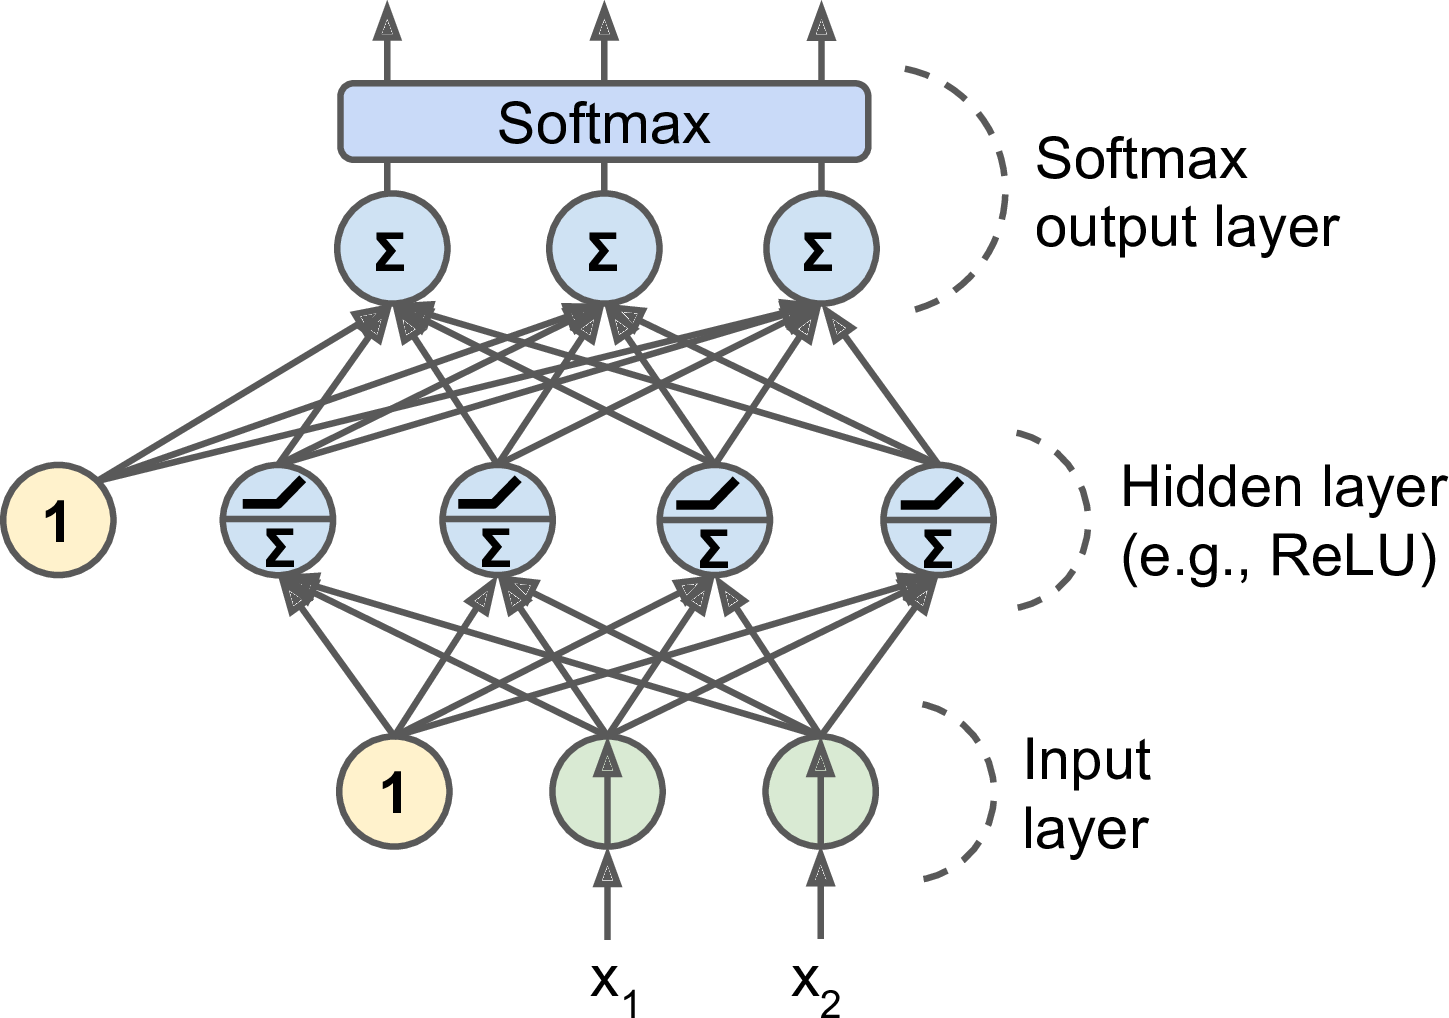
\includegraphics[width=0.50\textwidth]{./images/MLP_classification.png}
\end{figure}

%%%%%%%%%%%%%%%%%%%%%%%%%%%
%%%%%%%%%%%%%%%%%%%%%%%%%%%
%%%%%%%%%%%%%%%%%%%%%%%%%%%
%%%%%%%%%%%%%%%%%%%%%%%%%%%
%%%%%%%%%%%%%%%%%%%%%%%%%%%

\subsection{Implementing MLPs with Keras}

The following code creates a classification MLP with:
\vspace{-5.0mm}
\begin{itemize}
\item
An input layer with 784 neurons, where each instance is a $28*28$ array.
\vspace{-3.0mm}
\item
Two hidden layers (with 300 and 100 neurons, respectively).\newline
Both layers use the ReLU activation function.\newline
All the layers are connected sequentially.
\vspace{-3.0mm}
\item
10 exclusive classification outputs.
\end{itemize}

\vspace{-2.0mm}
\texttt{from tensorflow import keras}\newline
\texttt{model = keras.models.Sequential()}\newline
\texttt{model.add(keras.layers.Flatten(input\char`_shape=[28,28]))}\newline
\texttt{model.add(keras.layers.Dense(300, activation=\textquotesingle relu\textquotesingle))}\newline
\texttt{model.add(keras.layers.Dense(100, activation=\textquotesingle relu\textquotesingle))}\newline
\texttt{model.add(keras.layers.Dense(10, activation=\textquotesingle softmax\textquotesingle))}\newline
\vspace{-2.0mm}

For binary classification, use \texttt{activation=\textquotesingle sigmoid\textquotesingle} (i.e. the logistic function)\newline
For regression, the output layer would be:~\texttt{model.add(keras.layers.Dense(1))}

The following will give a summary of your model:\newline
\textit{Note that `None' in the Output Shape means that the batch size can be anything.}\newline
\texttt{model.summary()}

Each model layer is its own object:\newline
\texttt{input = model.layers[0]}\newline
\texttt{hidden\char`_1 = model.layers[1]}\newline
\texttt{hidden\char`_2 = model.layers[2]}\newline
\texttt{output = model.layers[3]}

Each layer manages its own connection weights between the layers neurons and their inputs:\newline
\texttt{weights, biases = hidden\char`_2.get\char`_weights()}

Notice that the connection weights are randomly initialized (this is required to break symmetry)
and the biases are initialized to zero.\newline
\textit{Sometimes you may want to use a different initialization method (information provided later).}

\newpage
\textbf{Compilation}\newline
After a model is created, you must specify the loss function and the optimizer to use:\newline
\texttt{model.compile(loss=\textquotesingle sparse\char`_categorical\char`_crossentropy\textquotesingle,}\newline
\texttt{.~~~~~~~~~~~~~optimizer=\textquotesingle sgd\textquotesingle,}\newline
\texttt{.~~~~~~~~~~~~~metrics=[\textquotesingle accuracy\textquotesingle]) \# these are optional}

For binary classification: \texttt{loss=\textquotesingle binary\char`_crossentropy\textquotesingle}\newline
For regression: \texttt{loss=\textquotesingle mean\char`_squared\char`_error\textquotesingle}

Note that the optimizer is equivalent to: \texttt{optimizer=keras.optimizers.SGD(lr=0.01)}\newline
\textit{Sometimes you may want to use more efficient optimizers (information provided later).}\newline

\textbf{Training}\newline
\texttt{history = model.fit(X, y, epochs=30, validation\char`_split=0.1)}

- The \texttt{fit()} method returns a History object containing meta-data about the training.\newline
- If not stated, the \texttt{epochs} parameter will default to one (not enough for convergence).\newline
- If not stated, the \texttt{validation\char`_split} parameter will be zero (i.e no cross validation).

Use the History object to plot the learning curves:\newline
\texttt{import pandas as pd}\newline
\texttt{import matplotlib.pyplot as plt}\newline
\texttt{pd.DataFrame(history.history).plot(figsize=(12,8))}\newline
\texttt{plt.grid(True)}\newline
\texttt{plt.gca().set\char`_ylim(0,1)}\newline
\texttt{plt.show()}\newline
\textit{Note that the validation error is computed at the \underline{end} of each epoch,
whilst the training error is computed using a running mean \underline{during} each epoch.}

To continue training, just call the \texttt{fit()} method again. Note the following:\newline
- This will create a new History object (rather than appending).\newline
- You can update the model compilation parameters before the additional training.\newline

\textbf{Evaluation}\newline
Estimate the generalization error using the test set:\newline
\texttt{model.evaluate(X\char`_test, y\char`_test)}

Make predictions as follows:\newline
\texttt{y\char`_proba = model.predict(X\char`_new)}\newline
\texttt{y\char`_pred ~= np.argmax(model.predict(X\char`_new), axis=-1)}\newline

\textbf{Saving and Loading}\newline
The following saves a model's architecture, parameters, and optimizer:\newline
\texttt{model.save(\textquotesingle my\char`_keras\char`_model.h5\textquotesingle)}

The following loads a model:\newline
\texttt{model = keras.models.load\char`_models(\textquotesingle model.h5\textquotesingle)}

You can also save your model at regular checkpoints during training...

\newpage
\textbf{Callbacks}\newline
The \texttt{fit()} method accepts a \textit{callbacks} argument
(a list of objects called \underline{during} training).

The following saves your model at regular intervals (default = end of each epoch):\newline
\texttt{save\char`_cb = keras.callbacks.ModelCheckpoint(\textquotesingle my\char`_keras\char`_model.h5\textquotesingle)}\newline
\texttt{history = model.fit(X, y, epochs=10, callbacks=[save\char`_cb])}

Moreover, if you use a validation set during training,
you can ensure your model only saves when the performance on the validation set is the best so far (i.e implicit early stopping):
\texttt{save\char`_cb = keras.callbacks.ModelCheckpoint(\textquotesingle my\char`_keras\char`_model.h5\textquotesingle,\newline
.~~~~~~~~~~~~~~~~~~~~~~~~~~~~~~~~~~~~~~~~~save\char`_best\char`_only=True)}\newline
\texttt{history = model.fit(X, y, epochs=100, validation\char`_split=0.1,\newline
.~~~~~~~~~~~~~~~~~~~callbacks=[save\char`_cb])}

Explicit early stopping can be implemented with the following callback:\newline
\texttt{early\char`_stop\char`_cb = \newline keras.callbacks.EarlyStopping(patience=10, restore\char`_best\char`_weights=True)}

%%%%%%%%%%%%%%%%%%%%%%%%%%%
%%%%%%%%%%%%%%%%%%%%%%%%%%%
%%%%%%%%%%%%%%%%%%%%%%%%%%%
%%%%%%%%%%%%%%%%%%%%%%%%%%%
%%%%%%%%%%%%%%%%%%%%%%%%%%%
\subsection{Fine-Tuning Neural Network Hyperparameters}

The flexibility of NNs is also one of their drawbacks,
there are many hyperparameters to tune:

\vspace{-5.0mm}
\begin{itemize}
\item
\textbf{Learning rate:} very low = $10^{-5}$, keras default = 0.01, very high = 10.\newline
\textit{Always retune this after changing another hyperparameter.}
\item
\textbf{Optimizer:} there are better options out there than mini-batch gradient descent...
\item
\textbf{Batch size:} keras default = 32 (large batch sizes can lead to training instabilities).
\item
\textbf{Hidden layer activation function:} ReLU is a good default in general.
\item
\textbf{Number of hidden layers:} for most problems, you can start with just one or two.
\item
\textbf{Number of neurons:} in general, use the same number for all hidden layers.\newline
\textit{It can sometimes help to make the first hidden layer bigger than the others.}
\item
\textbf{Keras Tuner:} use this library to tune hyperparameters \textit{(keras-team.github.io/keras-tuner/)}
\item
\textbf{Tip:} it's often simpler to pick a model with more layers and neurons than you actually need,
then use early stopping \& other regularization techniques to prevent overfitting.
\end{itemize}
% 
\textbf{Number of hidden layers}\newline
If it has enough neurons, one hidden layer can theoretically model the most complex functions.
% 
However, for complex problems,
deep networks have a much higher \textit{parameter efficiency} than shallow ones:
they can model complex functions using exponentially fewer neurons,
allowing them to reach much better performance with the same amount of training data.
% 
This is because real-world data is often structured in a hierarchial way,
and deep neural networks take advantage of this:\newline
- Lower hidden layers model low-level structures (e.g. line segments).\newline
- Intermediate hidden layers combine these to model intermediate-level structures (e.g. shapes).\newline
- The highest hidden layers combine these to model high-level structures (e.g. faces).\newline
- \textit{Transfer learning} is where you `borrow' the lower layers from a previously trained model.

\newpage
